% Options for packages loaded elsewhere
\PassOptionsToPackage{unicode}{hyperref}
\PassOptionsToPackage{hyphens}{url}
%
\documentclass[
]{article}
\usepackage{amsmath,amssymb}
\usepackage{iftex}
\ifPDFTeX
  \usepackage[T1]{fontenc}
  \usepackage[utf8]{inputenc}
  \usepackage{textcomp} % provide euro and other symbols
\else % if luatex or xetex
  \usepackage{unicode-math} % this also loads fontspec
  \defaultfontfeatures{Scale=MatchLowercase}
  \defaultfontfeatures[\rmfamily]{Ligatures=TeX,Scale=1}
\fi
\usepackage{lmodern}
\ifPDFTeX\else
  % xetex/luatex font selection
\fi
% Use upquote if available, for straight quotes in verbatim environments
\IfFileExists{upquote.sty}{\usepackage{upquote}}{}
\IfFileExists{microtype.sty}{% use microtype if available
  \usepackage[]{microtype}
  \UseMicrotypeSet[protrusion]{basicmath} % disable protrusion for tt fonts
}{}
\makeatletter
\@ifundefined{KOMAClassName}{% if non-KOMA class
  \IfFileExists{parskip.sty}{%
    \usepackage{parskip}
  }{% else
    \setlength{\parindent}{0pt}
    \setlength{\parskip}{6pt plus 2pt minus 1pt}}
}{% if KOMA class
  \KOMAoptions{parskip=half}}
\makeatother
\usepackage{xcolor}
\usepackage[margin=1in]{geometry}
\usepackage{graphicx}
\makeatletter
\def\maxwidth{\ifdim\Gin@nat@width>\linewidth\linewidth\else\Gin@nat@width\fi}
\def\maxheight{\ifdim\Gin@nat@height>\textheight\textheight\else\Gin@nat@height\fi}
\makeatother
% Scale images if necessary, so that they will not overflow the page
% margins by default, and it is still possible to overwrite the defaults
% using explicit options in \includegraphics[width, height, ...]{}
\setkeys{Gin}{width=\maxwidth,height=\maxheight,keepaspectratio}
% Set default figure placement to htbp
\makeatletter
\def\fps@figure{htbp}
\makeatother
\setlength{\emergencystretch}{3em} % prevent overfull lines
\providecommand{\tightlist}{%
  \setlength{\itemsep}{0pt}\setlength{\parskip}{0pt}}
\setcounter{secnumdepth}{-\maxdimen} % remove section numbering
\ifLuaTeX
  \usepackage{selnolig}  % disable illegal ligatures
\fi
\usepackage{bookmark}
\IfFileExists{xurl.sty}{\usepackage{xurl}}{} % add URL line breaks if available
\urlstyle{same}
\hypersetup{
  hidelinks,
  pdfcreator={LaTeX via pandoc}}

\author{}
\date{\vspace{-2.5em}}

\begin{document}

\documentclass{article}
\usepackage{graphicx}
\usepackage{float}
\usepackage{geometry}
\geometry{margin=1in}

\title{Billionaires' Net Worth Analysis}
\author{Stanley Osei-Wusu (GH1021715)}
\date{\today}

\begin{document}

\maketitle
\newpage

\tableofcontents
\newpage

\section{Introduction}
This report presents a comprehensive dataset analysis containing information about 2,640 billionaires, including their net worth, age, gender, country of residence, industry, and other relevant socio-economic factors. The study aimed to explore patterns in the distribution of net worth, investigate relationships between net worth and other variables such as age and industry, and perform regression and hypothesis testing to identify potential predictors of net worth.

\newpage
\section{Data Cleaning and Preparation}
Before conducting the analysis, several data cleaning steps were performed to ensure the integrity and usability of the data:

\begin{itemize}
    \item \textbf{Missing Values Imputation}: Missing values in age and other numeric columns were imputed using the median or mean, as appropriate. 
    \item \textbf{Conversion to Numeric Values}: The \texttt{finalWorth} column, representing the net worth in millions, contained non-numeric characters. These were removed to convert the column into a numeric format.
    \item \textbf{Categorical Data Conversion}: Categorical variables such as \texttt{gender}, \texttt{category}, and \texttt{residenceStateRegion} were converted to factors for better handling in statistical analysis.
    \item \textbf{Data Filtering}: Rows with missing or zero values in critical variables, such as \texttt{finalWorth}, were removed.
\end{itemize}

\newpage
\section{Exploratory Data Analysis (EDA)}

\subsection{Distribution of Net Worth}
The net worth of billionaires ranged from \$1 billion to \$211 billion. The median net worth was approximately \$2.3 billion, and the mean was around \$4.6 billion, indicating a right-skewed distribution where a few extremely wealthy individuals significantly increased the mean.

\begin{figure}[H]
    \centering
    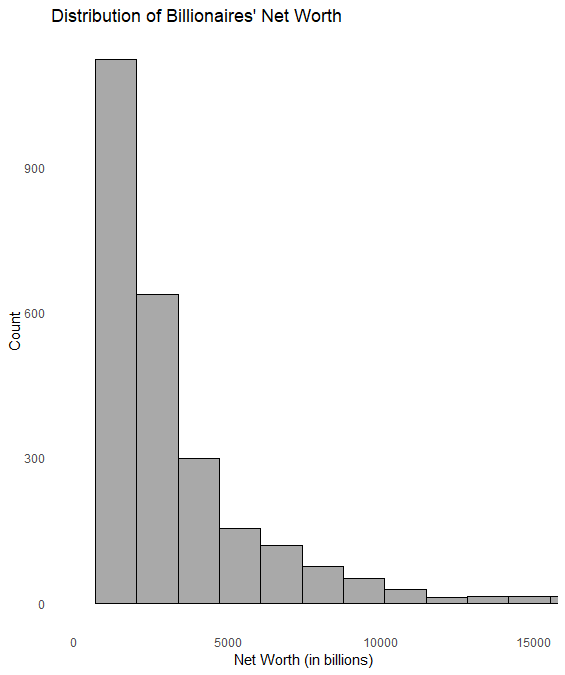
\includegraphics[width=\textwidth]{Distribution of Billionaire Net Worth.png}
    \caption{Distribution of Billionaires' Net Worth}
\end{figure}

\subsection{Scatter Plot - Age vs. Net Worth}
A scatter plot of age against net worth revealed a weak positive relationship between age and net worth, suggesting that older individuals tend to accumulate more wealth. However, the relationship was not strong, indicating that age alone is not a significant predictor of net worth.

\begin{figure}[H]
    \centering
    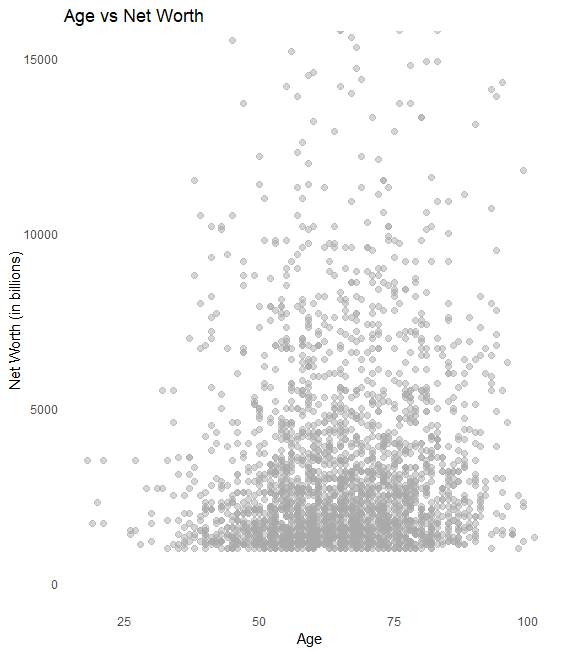
\includegraphics[width=\textwidth]{Rplot02.png}
    \caption{Age vs Net Worth}
\end{figure}

\subsection{Net Worth Distribution by Industry}
The box plot below shows the distribution of net worth across different industries, revealing substantial variation. Industries like "Energy" and "Finance \& Investments" show wider ranges and higher medians.

\begin{figure}[H]
    \centering
    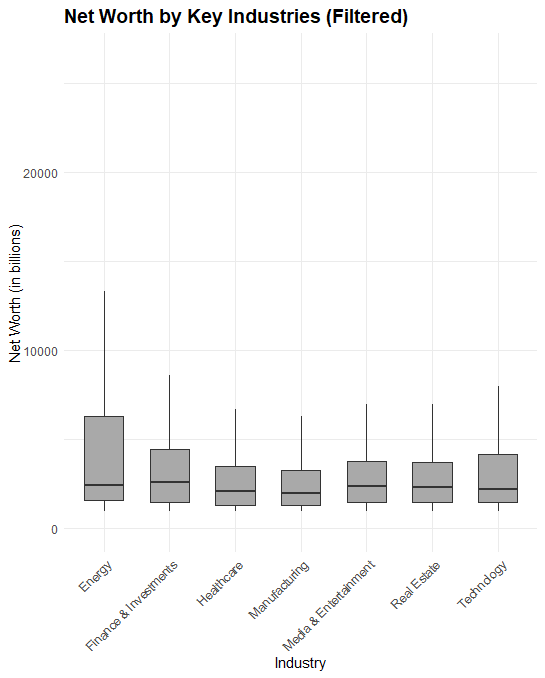
\includegraphics[width=\textwidth]{Rplot05.png}
    \caption{Net Worth by Key Industries (Filtered)}
\end{figure}

\subsection{Average Net Worth by Gender}
The bar plot of average net worth by gender indicates that male billionaires have a slightly higher average net worth compared to female billionaires.

\begin{figure}[H]
    \centering
    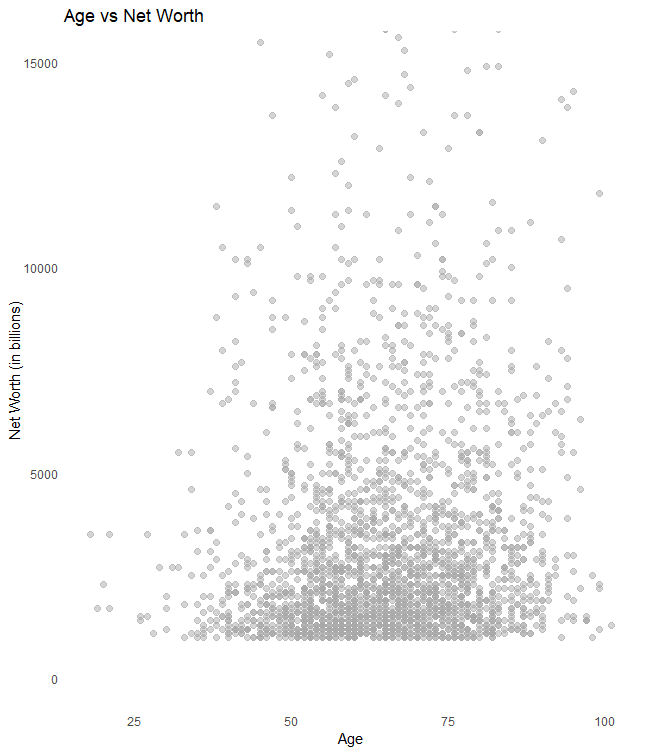
\includegraphics[width=\textwidth]{Rplot01.png}
    \caption{Average Net Worth by Gender}
\end{figure}

\newpage
\section{Hypothesis Testing}
To test the relationships between variables, the following hypotheses were set up:

\begin{itemize}
    \item \textbf{H0 (Null Hypothesis)}: There is no significant relationship between age, industry, or gender and the net worth of billionaires.
    \item \textbf{H1 (Alternative Hypothesis)}: There is a significant relationship between age, industry, or gender and the net worth of billionaires.
\end{itemize}

Results of the Welch Two Sample t-test for gender and net worth are as follows:

\begin{verbatim}
    Welch Two Sample t-test
    data: finalWorth by gender
    t = 0.77808, df = 422.13, p-value = 0.437
    alternative hypothesis: true difference in means between group F and group M is not equal to 0
    95 percent confidence interval: -336.5730  777.6321
    sample estimates:
    mean in group F mean in group M 
       4023.952        3803.423 
\end{verbatim}

Based on the p-value of 0.437, we fail to reject the null hypothesis, meaning that there is no significant difference in net worth between male and female billionaires.

\newpage
\section{Regression Analysis}
A multiple linear regression analysis was performed to identify the factors influencing billionaires' net worth. The regression model included the following predictors: age, gender, industry, and country.

\subsection{Model Summary}
The model's Adjusted R-squared was 0.075, indicating that the model explains about 7.5\% of the variance in net worth.

\subsection{Diagnostics}
\begin{figure}[H]
    \centering
    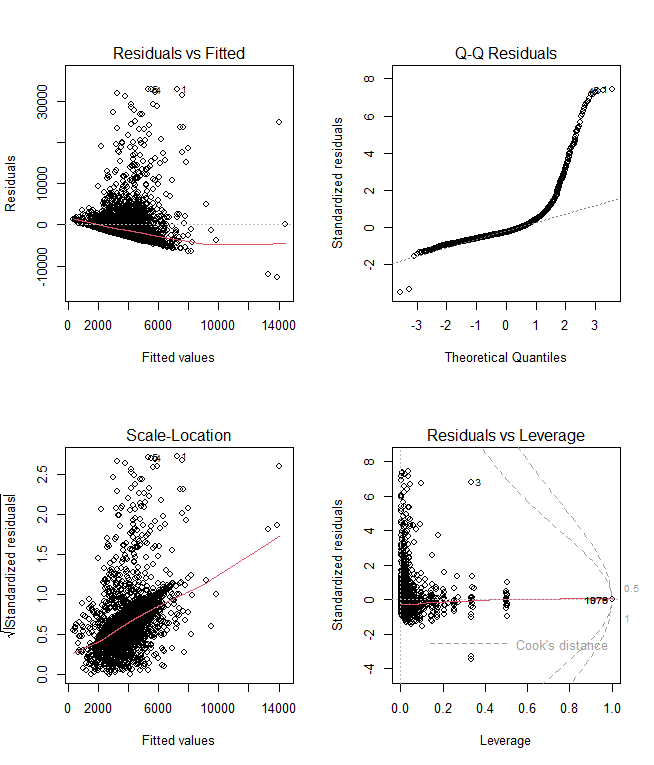
\includegraphics[width=\textwidth]{Rplot07.png}
    \caption{Regression Diagnostics: Residuals vs Fitted, Q-Q Plot, and More}
\end{figure}

\newpage
\section{Logistic Regression Analysis}
A logistic regression model was applied to predict whether a billionaire belongs to the "Technology" industry based on their age, gender, and net worth.

\subsection{ROC Curve}
\begin{figure}[H]
    \centering
    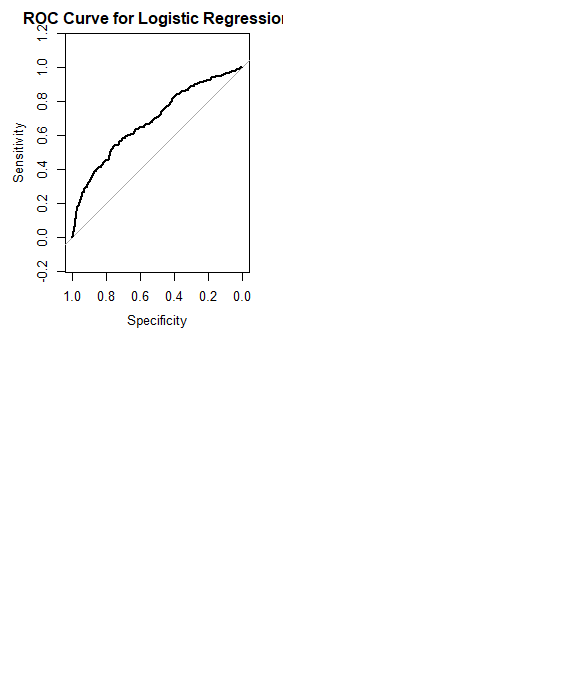
\includegraphics[width=\textwidth]{Rplot08.png}
    \caption{ROC Curve for Logistic Regression}
\end{figure}

\newpage
\section{Conclusion}
The analysis provided insights into the distribution and determinants of billionaires' net worth:

\begin{itemize}
    \item The net worth distribution is highly skewed, with a few individuals holding a significant proportion of the wealth.
    \item Age and industry are significant predictors of net worth, but the overall explanatory power of these variables is limited.
    \item Gender does not appear to be a significant factor in determining net worth among billionaires.
\end{itemize}

\end{document}

\end{document}
